%%%%%%%%%%%%%%%%%%%%%%%%%%%%%%%%%%%%%%%%%%%%%%%%%%%%%%%%%%%%%%%%%%%%%%%%%%%%%%%%%%%%%
%																					%
%	TRABAJO: Paper Redes de Petri Temporizadas										%
%																					%
%		Titulo: 	Ejecucion de Redes de Petri Temporizadas						%
%																					%
%		Autores:	Julian Nonino													%
%					Carlos Renzo Pisetta											%
%					Orlando Micolini												%
%																					%
%	Seccion: Biografias																%	
%	Archivo: biografias.tex															%
%																					%
%%%%%%%%%%%%%%%%%%%%%%%%%%%%%%%%%%%%%%%%%%%%%%%%%%%%%%%%%%%%%%%%%%%%%%%%%%%%%%%%%%%%%
%	REVISIONES																		%
%																					%
%		18/10/2012																	%
%			Julian Nonino															%
%				Creacion de este archivo											%
%		18/10/2012																	%
%			Renzo Pisetta															%	
%				Codificacion de esta seccion										%
%		04/04/2013																	%
%			Julian Nonino															%
%				Actualizacion 														%		
%																					%
%%%%%%%%%%%%%%%%%%%%%%%%%%%%%%%%%%%%%%%%%%%%%%%%%%%%%%%%%%%%%%%%%%%%%%%%%%%%%%%%%%%%%

% biography section
% 
% If you have an EPS/PDF photo (graphicx package needed) extra braces are
% needed around the contents of the optional argument to biography to prevent
% the LaTeX parser from getting confused when it sees the complicated
% \includegraphics command within an optional argument. (You could create
% your own custom macro containing the \includegraphics command to make things
% simpler here.)
%\begin{biography}[{\includegraphics[width=1in,height=1.25in,clip,keepaspectratio]{./jnonino.png}}]{Juli�n Nonino}
% or if you just want to reserve a space for a photo:


\begin{IEEEbiography}[{\includegraphics[width=1in,height=1.25in,clip,keepaspectratio]{./img/jnonino.png}}]{Juli�n Nonino}
(M'2011) naci� en Rio Cuarto, C�rdoba, Argentina el d�a 16 de octubre de 1988. En el a�o 2012 obtuvo 
el t�tulo de grado Ingeniero en Computaci�n de la Facultad de Ciencias Exactas, F�sicas y Naturales 
de la Universidad Nacional de C�rdoba.
Actualmente se desempe�a como Ingeniero de Software en Motorola Mobility of Argentina S.A. 
En el ambito universitario, precisamente en la Facultad de Ciencias Exactas, F�sicas y Naturales de 
la Universidad Nacional de C�rdoba, colabora en las c�tedras Ingenier�a de Software y Gesti�n de la 
Calidad de Software. Tambi�n, en el Laboratorio de Arquitectura de Computadoras de la misma universidad, 
realiza actividades relacionadas con el dise�o e implementaci�n de software y hardware optimizado 
para sistemas de computaci�n en paralelo basados en Redes de Petri.
\end{IEEEbiography}

\begin{IEEEbiography}[{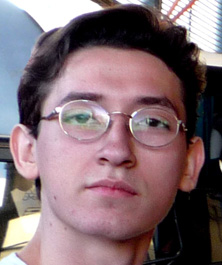
\includegraphics[width=1in,height=1.25in,clip,keepaspectratio]{./img/crpisetta}}]{Carlos Renzo Pisetta}
(M'2011) naci� en C�rdoba, Argentina el d�a 07 de junio de 1989. En el a�o 2012 obtuvo 
el t�tulo de grado Ingeniero en Computaci�n de la Facultad de Ciencias Exactas, F�sicas y Naturales 
de la Universidad Nacional de C�rdoba.
Actualmente se desempe�a como investigador en el Laboratorio de Arquitectura de Computadoras en la UNC(FCEFyN) abocado 
al dise�o e implementaci�n de software y hardware optimizado para sistemas de computaci�n en paralelo basados en Redes de Petri.
\end{IEEEbiography}

\begin{IEEEbiography}[{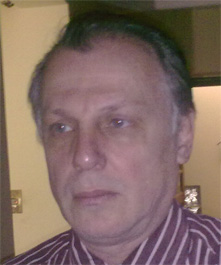
\includegraphics[width=1in,height=1.25in,clip,keepaspectratio]{./img/omicolini}}]{Orlando Micolini}
Grado en Ingeniero Electricista Electr�nico, a�o 1981, de la UNC (FCEFyN) Argentina. Postgrado Especialista en Telecomunicaciones,
a�o 2002, de la UNC (FCEFyN) Argentina. Mag�ster en Ciencias de la Ingenier�a, a�o 2002, de la UNC (FCEFyN) Argentina.
Director de SCS S.R.L, desde 1991 a 2008. Director de la Carrera de Ingenier�a en Computaci�n en la  UNC (FCEFyN) Argentina
(2004-actualidad). Titular de la asignatura Arquitectura de Computadoras en la  UNC (FCEFyN) Argentina (1996-actualidad). 
Actualmente est� trabajando, realizando el doctorado de Ciencias Inform�tica en la Universidad Nacional de la Plata, 
en sistemas multi-core heterog�neos con Redes de Petri.
\end{IEEEbiography}

% You can push biographies down or up by placing
% a \vfill before or after them. The appropriate
% use of \vfill depends on what kind of text is
% on the last page and whether or not the columns
% are being equalized.
%	\vfill
	
% Can be used to pull up biographies so that the bottom of the last one
% is flush with the other column.
%\enlargethispage{-5in}